\documentclass[
  shownotes,
  xcolor={svgnames},
  hyperref={colorlinks,citecolor=DarkBlue,linkcolor=DarkRed,urlcolor=DarkBlue}
  ]{beamer}
\usepackage{animate}
\usepackage{amsmath}
\usepackage{amsfonts}
\usepackage{amssymb}
\usepackage{pifont}
\usepackage{mathpazo}
%\usepackage{xcolor}
\usepackage{multimedia}
\usepackage{fancybox}
\usepackage[para]{threeparttable}
\usepackage{multirow}
\setcounter{MaxMatrixCols}{30}
\usepackage{subcaption}
\usepackage{graphicx}
\usepackage{lscape}
\usepackage[compatibility=false,font=small]{caption}
\usepackage{booktabs}
\usepackage{ragged2e}
\usepackage{chronosys}
\usepackage{appendixnumberbeamer}
\usepackage{animate}
\setbeamertemplate{caption}[numbered]
\usepackage{color}
%\usepackage{times}
\usepackage{tikz}
\usepackage{comment} %to comment
%% BibTeX settings
\usepackage{natbib}
\bibliographystyle{apalike}
\bibpunct{(}{)}{,}{a}{,}{,}
\setbeamertemplate{bibliography item}{[\theenumiv]}

% Defines columns for bespoke tables
\usepackage{array}
\newcolumntype{L}[1]{>{\raggedright\let\newline\\\arraybackslash\hspace{0pt}}m{#1}}
\newcolumntype{C}[1]{>{\centering\let\newline\\\arraybackslash\hspace{0pt}}m{#1}}
\newcolumntype{R}[1]{>{\raggedleft\let\newline\\\arraybackslash\hspace{0pt}}m{#1}}


\usepackage{xfrac}


\usepackage{multicol}
\setlength{\columnsep}{0.5cm}

% Theme and colors
\usetheme{Boadilla}

% I use steel blue and a custom color palette. This defines it.
\definecolor{andesred}{HTML}{af2433}

% Other options
\providecommand{\U}[1]{\protect\rule{.1in}{.1in}}
\usefonttheme{serif}
\setbeamertemplate{itemize items}[default]
\setbeamertemplate{enumerate items}[square]
\setbeamertemplate{section in toc}[circle]

\makeatletter

\definecolor{mybackground}{HTML}{82CAFA}
\definecolor{myforeground}{HTML}{0000A0}

\setbeamercolor{normal text}{fg=black,bg=white}
\setbeamercolor{alerted text}{fg=red}
\setbeamercolor{example text}{fg=black}

\setbeamercolor{background canvas}{fg=myforeground, bg=white}
\setbeamercolor{background}{fg=myforeground, bg=mybackground}

\setbeamercolor{palette primary}{fg=black, bg=gray!30!white}
\setbeamercolor{palette secondary}{fg=black, bg=gray!20!white}
\setbeamercolor{palette tertiary}{fg=white, bg=andesred}

\setbeamercolor{frametitle}{fg=andesred}
\setbeamercolor{title}{fg=andesred}
\setbeamercolor{block title}{fg=andesred}
\setbeamercolor{itemize item}{fg=andesred}
\setbeamercolor{itemize subitem}{fg=andesred}
\setbeamercolor{itemize subsubitem}{fg=andesred}
\setbeamercolor{enumerate item}{fg=andesred}
\setbeamercolor{item projected}{bg=gray!30!white,fg=andesred}
\setbeamercolor{enumerate subitem}{fg=andesred}
\setbeamercolor{section number projected}{bg=gray!30!white,fg=andesred}
\setbeamercolor{section in toc}{fg=andesred}
\setbeamercolor{caption name}{fg=andesred}
\setbeamercolor{button}{bg=gray!30!white,fg=andesred}


\usepackage{fancyvrb}
\newcommand{\VerbBar}{|}
\newcommand{\VERB}{\Verb[commandchars=\\\{\}]}
\DefineVerbatimEnvironment{Highlighting}{Verbatim}{commandchars=\\\{\}}
% Add ',fontsize=\small' for more characters per line
\usepackage{framed}
\definecolor{shadecolor}{RGB}{248,248,248}
\newenvironment{Shaded}{\begin{snugshade}}{\end{snugshade}}
\newcommand{\AlertTok}[1]{\textcolor[rgb]{0.94,0.16,0.16}{#1}}
\newcommand{\AnnotationTok}[1]{\textcolor[rgb]{0.56,0.35,0.01}{\textbf{\textit{#1}}}}
\newcommand{\AttributeTok}[1]{\textcolor[rgb]{0.77,0.63,0.00}{#1}}
\newcommand{\BaseNTok}[1]{\textcolor[rgb]{0.00,0.00,0.81}{#1}}
\newcommand{\BuiltInTok}[1]{#1}
\newcommand{\CharTok}[1]{\textcolor[rgb]{0.31,0.60,0.02}{#1}}
\newcommand{\CommentTok}[1]{\textcolor[rgb]{0.56,0.35,0.01}{\textit{#1}}}
\newcommand{\CommentVarTok}[1]{\textcolor[rgb]{0.56,0.35,0.01}{\textbf{\textit{#1}}}}
\newcommand{\ConstantTok}[1]{\textcolor[rgb]{0.00,0.00,0.00}{#1}}
\newcommand{\ControlFlowTok}[1]{\textcolor[rgb]{0.13,0.29,0.53}{\textbf{#1}}}
\newcommand{\DataTypeTok}[1]{\textcolor[rgb]{0.13,0.29,0.53}{#1}}
\newcommand{\DecValTok}[1]{\textcolor[rgb]{0.00,0.00,0.81}{#1}}
\newcommand{\DocumentationTok}[1]{\textcolor[rgb]{0.56,0.35,0.01}{\textbf{\textit{#1}}}}
\newcommand{\ErrorTok}[1]{\textcolor[rgb]{0.64,0.00,0.00}{\textbf{#1}}}
\newcommand{\ExtensionTok}[1]{#1}
\newcommand{\FloatTok}[1]{\textcolor[rgb]{0.00,0.00,0.81}{#1}}
\newcommand{\FunctionTok}[1]{\textcolor[rgb]{0.00,0.00,0.00}{#1}}
\newcommand{\ImportTok}[1]{#1}
\newcommand{\InformationTok}[1]{\textcolor[rgb]{0.56,0.35,0.01}{\textbf{\textit{#1}}}}
\newcommand{\KeywordTok}[1]{\textcolor[rgb]{0.13,0.29,0.53}{\textbf{#1}}}
\newcommand{\NormalTok}[1]{#1}
\newcommand{\OperatorTok}[1]{\textcolor[rgb]{0.81,0.36,0.00}{\textbf{#1}}}
\newcommand{\OtherTok}[1]{\textcolor[rgb]{0.56,0.35,0.01}{#1}}
\newcommand{\PreprocessorTok}[1]{\textcolor[rgb]{0.56,0.35,0.01}{\textit{#1}}}
\newcommand{\RegionMarkerTok}[1]{#1}
\newcommand{\SpecialCharTok}[1]{\textcolor[rgb]{0.00,0.00,0.00}{#1}}
\newcommand{\SpecialStringTok}[1]{\textcolor[rgb]{0.31,0.60,0.02}{#1}}
\newcommand{\StringTok}[1]{\textcolor[rgb]{0.31,0.60,0.02}{#1}}
\newcommand{\VariableTok}[1]{\textcolor[rgb]{0.00,0.00,0.00}{#1}}
\newcommand{\VerbatimStringTok}[1]{\textcolor[rgb]{0.31,0.60,0.02}{#1}}
\newcommand{\WarningTok}[1]{\textcolor[rgb]{0.56,0.35,0.01}{\textbf{\textit{#1}}}}
\usepackage{graphicx}
\makeatletter

\definecolor{airforceblue}{rgb}{0.36, 0.54, 0.66}

\usepackage{tikz}
% Tikz settings optimized for causal graphs.
\usetikzlibrary{shapes,decorations,arrows,calc,arrows.meta,fit,positioning}
\tikzset{
    -Latex,auto,node distance =1 cm and 1 cm,semithick,
    state/.style ={ellipse, draw, minimum width = 0.7 cm},
    point/.style = {circle, draw, inner sep=0.04cm,fill,node contents={}},
    bidirected/.style={Latex-Latex,dashed},
    el/.style = {inner sep=2pt, align=left, sloped}
}


\makeatother






%%%%%%%%%%%%%%% BEGINS DOCUMENT %%%%%%%%%%%%%%%%%%

\begin{document}

\title[Lecture 14]{Lecture 14: \\ Overfit \& Cross Validation}
\subtitle{Big Data and Machine Learning for Applied Economics \\ Econ 4676}
\date{\today}

\author[Sarmiento-Barbieri]{Ignacio Sarmiento-Barbieri}
\institute[Uniandes]{Universidad de los Andes}


\begin{frame}[noframenumbering]
\maketitle
\end{frame}

%%%%%%%%%%%%%%%%%%%%%%%%%%%%%%%%%%%

%----------------------------------------------------------------------%
\begin{frame}
\frametitle{Announcements \& Recap}

\begin{itemize}
  \item Final Project
  \medskip
  \begin{itemize}
    \item First deadline. Sept 25.  Brief zoom hang out, short presentation (5 slides tops). Present idea and basic plan. \textcolor{airforceblue}{soft deadline}
     \medskip
    \item  Second deadline. October 25. Show data. \textcolor{andesred}{hard deadline}
      \medskip
    \item  Final work, December 17. Bonus for ``complete papers'' \textcolor{andesred}{hard deadline}
  \end{itemize}
\bigskip   
  \item Details on Spatial Lag Model
  \medskip
      \begin{itemize} 
        \item MLE
            \medskip
        \item 2SLS
      \end{itemize}
\end{itemize}

\end{frame}

%----------------------------------------------------------------------% 

\begin{frame}
\frametitle{Agenda}

\tableofcontents

\end{frame}

%----------------------------------------------------------------------%
\section{Motivation }
%----------------------------------------------------------------------%
\begin{frame}[fragile]
\frametitle{Motivation: Back to Basics}
\framesubtitle{Complexity and the variance/bias trade off}

\begin{itemize}

  \item When the focus switches from estimating $f$ to predicting $Y$, 
  \medskip
  \item $f$ plays a secondary role, as just a tool to improve the prediction based on $X$.
  \medskip
  \item  Predicting $Y$ involves \emph{learning} $f$, that is, $f$ is no longer taken as given, as in the classical view. 
  \medskip
  \item Now it implies an iterative process where initial choices for $f$ are revised in light of potential improvements in predictive performance.
  \medskip
  \item Model choice or learning involves choosing both $f$ and a strategy to estimate it ($\hat f$), guided by predictive performance. 

\end{itemize}


\end{frame}

%----------------------------------------------------------------------%
\begin{frame}
\frametitle{Complexity and the variance/bias trade off}



\begin{equation}
Y=\beta_1 X_1 + \beta_2 X_2 + u_2
\end{equation}

\bigskip
\begin{itemize}
  \item Omitting relevant variables, vs including irrelevant variables
  \item Trade off: more {\it complex} models tend to have less bias but higher variance
  \item Complexity: number of variables?
  \item Classical econometrics: first unbiasedness
  \item ML: Accept some bias to lower variance
\end{itemize}

\end{frame}
%----------------------------------------------------------------------%
\section{Overfit}
%----------------------------------------------------------------------%
\begin{frame}[fragile]
\frametitle{Overfit}


        \begin{figure}[H] \centering
            \captionsetup{justification=centering}
              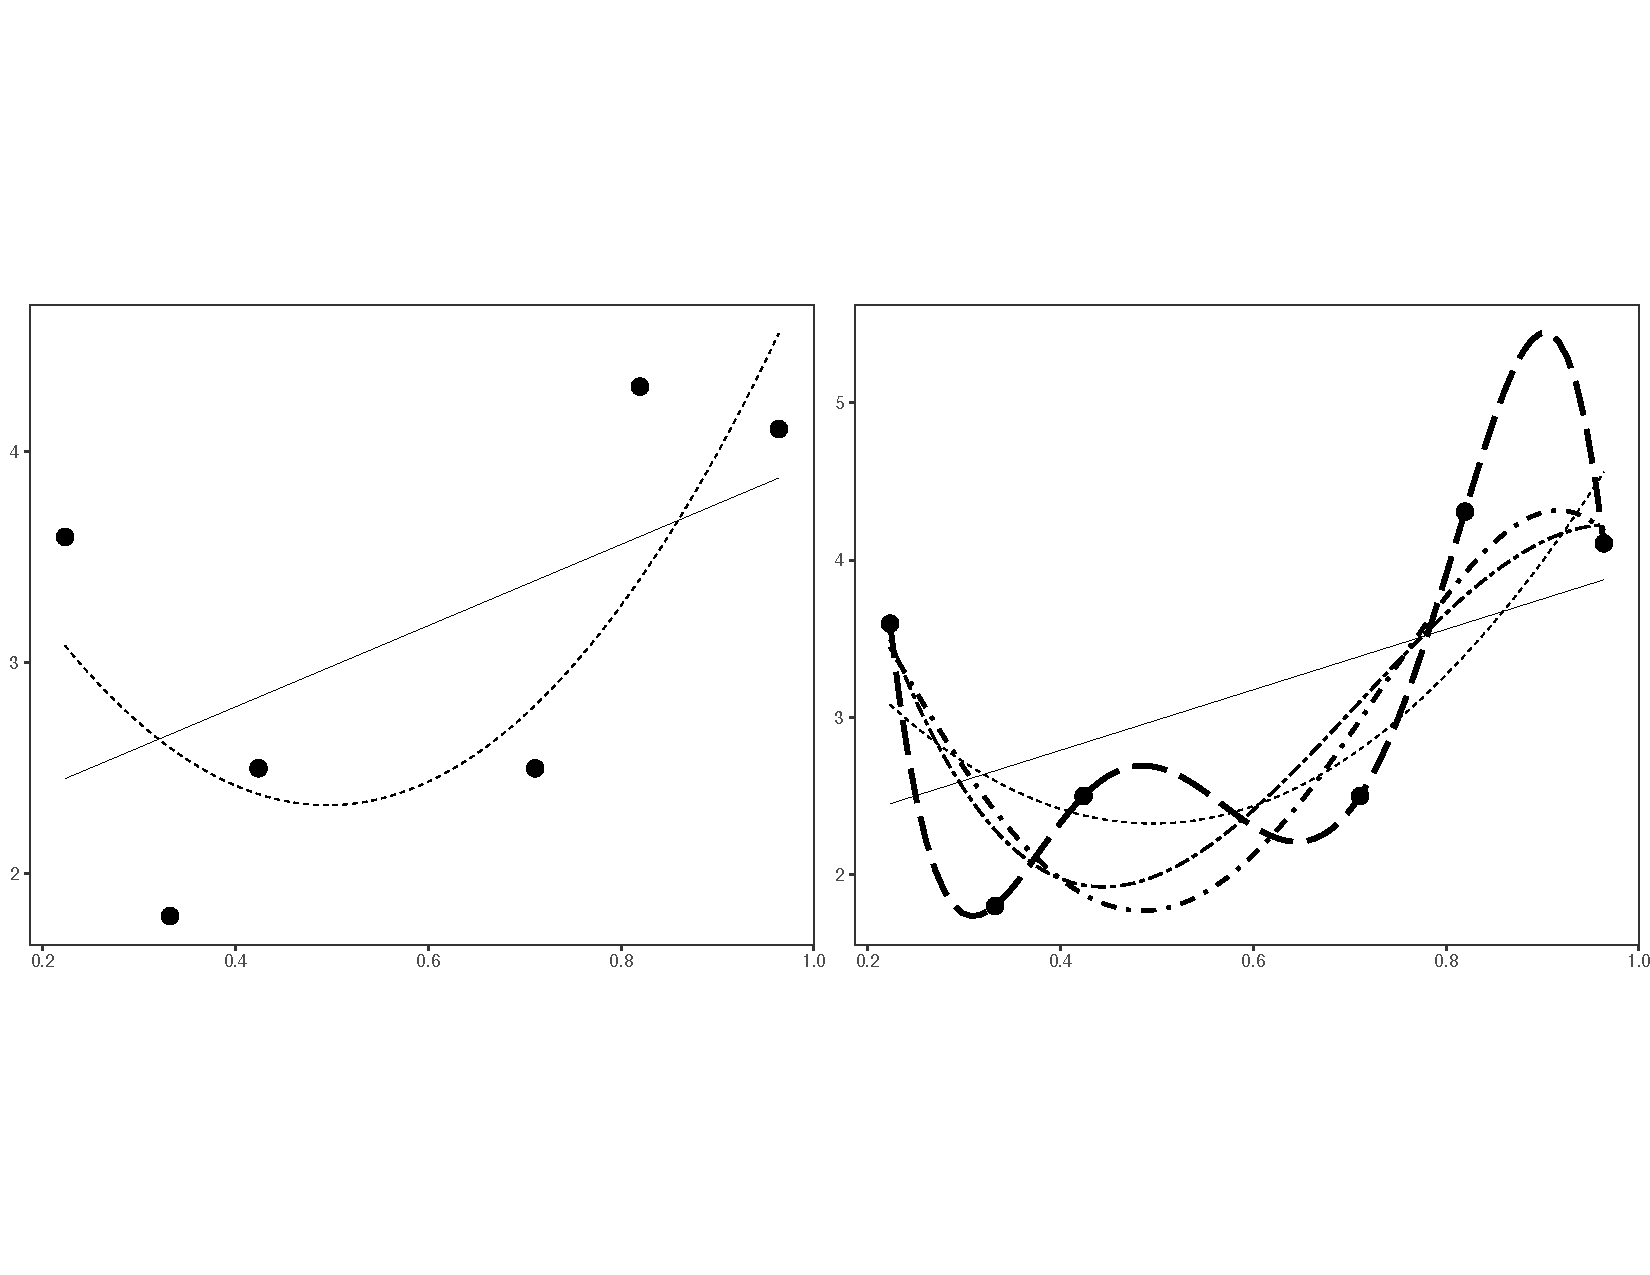
\includegraphics[scale=0.4]{figures/fig_1a.pdf}
 \end{figure}


\end{frame}

%----------------------------------------------------------------------%
\begin{frame}[fragile]
\frametitle{Overfit}


\begin{itemize}

  \item Suppose that the true model is $y=f(X) +u$ where $f$ is a polynomial of degree $p^*$, with $E(u)=0$ and $V(u)=\sigma^2$
  \medskip
  \item $p^*$ is finite but unknown
  \medskip
  \item  We fit polynomials with increasing degrees $p=1,2,....$
  \medskip
  \item What happens when we increase the degree of the polynomial?
  \medskip
  \item The expected prediction error of a regression fit $\hat f(X)$ at an input point $X=x_0$, is

  \begin{align}
  Err(x_0)&=Err(y-\hat f(x_0)|X=x_0) \nonumber \\
          &= Bias^2 (f,\hat f(x_0)) + V(\hat f(x_0)) + Irreducible\,Error
  \end{align}
\item The average expected prediction error

\begin{flushleft}
\begin{align}
  \frac{1}{N} \sum _{i=1}^N Err(x_i) 
  \end{align}
\end{flushleft}
  
\end{itemize}

\end{frame}

%----------------------------------------------------------------------%
\begin{frame}[fragile]
\frametitle{Overfit}


\begin{itemize}

  \item Bias ?
  \item Variance:
\end{itemize}

  \begin{align}
  \hat f(x_0) = \sum_{s=0}^p x_0^s\hat\beta_s = x_0'\hat\beta  
  \end{align}

  where $x_0'=(1,x_0,,x_0^2,\dots,x_0^p)$

  \begin{align}
  V(\hat f(x_0) ) = V(x_0'\hat\beta) = x_0'\sigma^2(X'X)^{-1}x_0
  \end{align}

  Then 

  \begin{align}
\frac{1}{n}\sum_{i=1}^n\sigma^2 x_{i}'\sigma^2(X'X)^{-1}x_{i}= \sigma^2 \frac{p}{n}
\end{align}


After we "hit" $p^*$ increasing complexity does not reduce the bias, but variance increases monotonically for $\sigma^2$ and $n$ given
 


\end{frame}

%----------------------------------------------------------------------%
\begin{frame}[fragile]
\frametitle{Proof}


The fitted model for a polynomial of degree $p$ is :
\begin{align}
\hat y_i = x_i'\hat\beta  
\end{align}
with  $x_i'=(1,x_i,,x_i^2,\dots,x_i^p)$
Then $V(y_i) = V(x_i'\hat\beta)= \sigma^2 x_i'(X'X)^{-1}x_i$. Now:

\begin{align}
Average\, V(x_i'\hat \beta)=\frac{1}{n}\sum_{i=1}^n \sigma^2 x_i'(X'X)^{-1}x_i
\end{align}

\end{frame}
%----------------------------------------------------------------------%
\begin{frame}[fragile]
\frametitle{Proof}

\begin{scriptsize}
\begin{Shaded}
\begin{itemize}
  \item Trace.
  \begin{itemize}
    \tiny
  \item If $A_{m\times m}$ with typical element $a_{ij}$. The {\bf trace} of A, $tr(A)$ is the sum of the elements of its diagonal: $tr(A)\equiv \sum_{s=1}^m a_{ii}$
  \item Properties
  \begin{itemize}
    \tiny
    \item For any square matrices A, B, and C: $tr(A+B)=tr(A)+tr(B)$
    \item Cyclic property: $tr(ABC)=tr(BCA)=tr(CAB)$
    \item If $m=1$ tr(A)=A
  \end{itemize}
  \end{itemize}
\end{itemize}
\end{Shaded}
\end{scriptsize}
Now we use traces. Note that $x_i'(X'X)^{-1}x_i$ is a scalar, using the third property of traces

\begin{align}
Average\,V(x_i'\hat \beta)=\frac{1}{n}\sum_{i=1}^n \sigma^2 x_i'(X'X)^{-1}x_i)
\end{align}

Now, using the cyclic property, $tr(x_i'(X'X)^{-1}x_i)=tr((X'X)^{-1}x_i'x_i)$, and using the first property of traces, we get

\begin{align}
\sum_{i=1}^n tr((X'X)^{-1}x_i'x_i) = tr(\sum_{i=1}^n (X'X)^{-1}x_i'x_i) =tr ((X'X)^{-1}(X'X)) = p
\end{align}

\end{frame}
%----------------------------------------------------------------------%
\subsection{Overfit and out of Sample Prediction}
%----------------------------------------------------------------------%
\begin{frame}[fragile]
\frametitle{Overfit and out of Sample Prediction}


\begin{itemize}
  \item ML we care about prediction out of sample
  \medskip
  \item Overfit: complex models predict very well inside a sample but "bad" outside
  \medskip
  \item Choose the right complexity level
  \medskip
  \item How do we measure the out of sample error?
  \medskip
  \item $R^2$ doesn't work: measures prediction in sample, it's non decreasing in complexity (PS1)
\end{itemize}

\end{frame}
%----------------------------------------------------------------------%
\begin{frame}[fragile]
\frametitle{Overfit and out of Sample Prediction}


        \begin{figure}[H] \centering
            \captionsetup{justification=centering}
              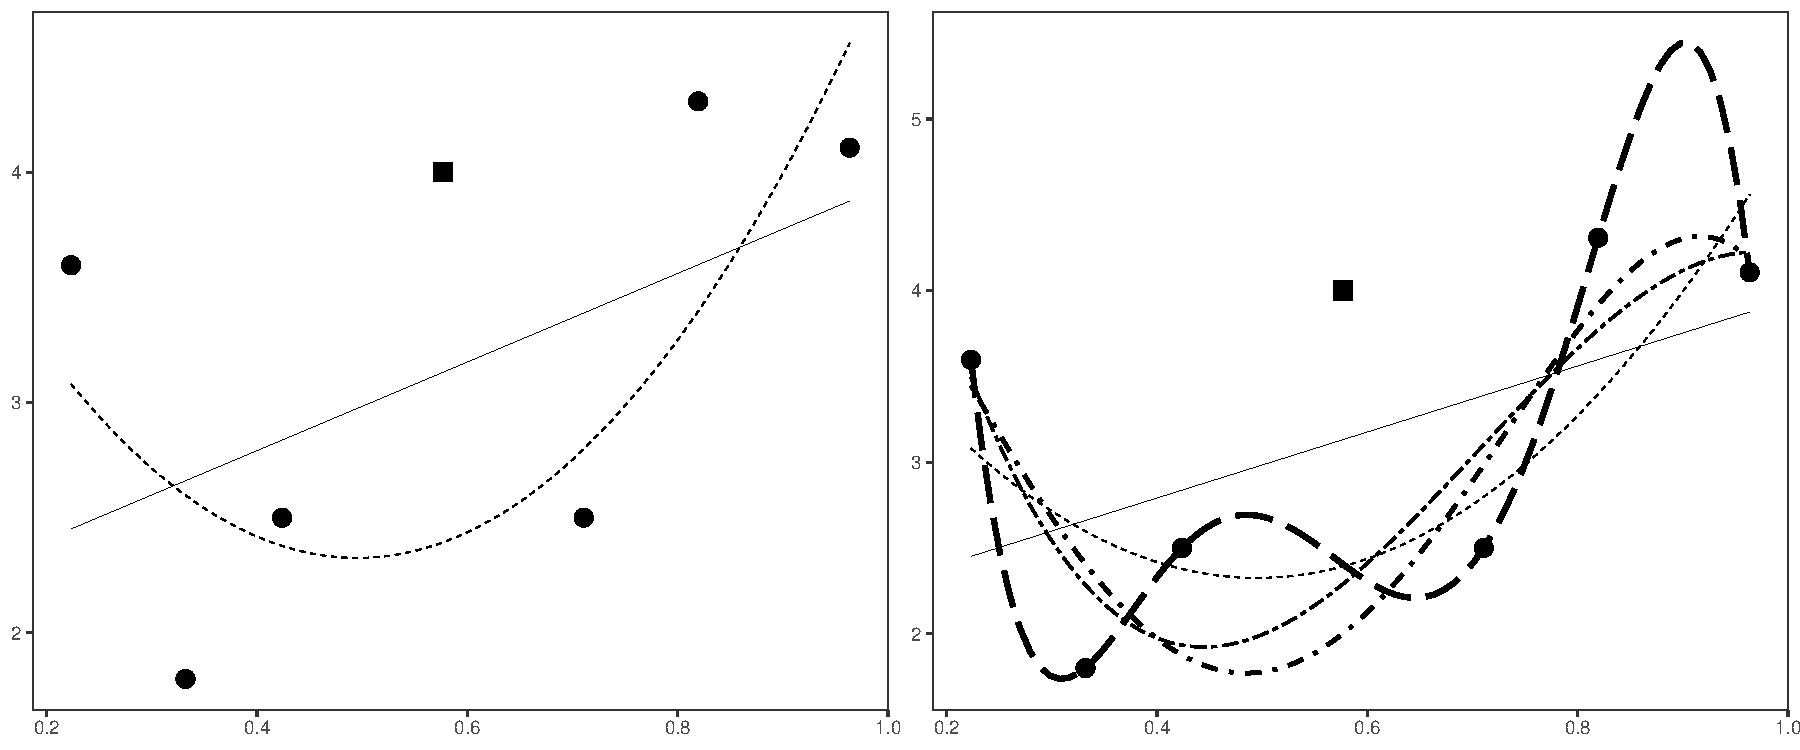
\includegraphics[scale=0.4]{figures/fig_1b.pdf}
 \end{figure}

\end{frame}
%----------------------------------------------------------------------%
\begin{frame}[fragile]
\frametitle{Overfit and out of Sample Prediction}

\begin{itemize}
\item Recall from Lecture 2 we defined loss and risk functions
\begin{itemize}
  \item Squared Error Loss $L(y,\hat y) =(y-\hat y)^2$
  \item Risk function $E(L(y,\hat y))$ that we also call expected prediction error (or sample counterpart average prediction error)

\end{itemize}
\item Now we introduce formally two new/old concepts
\begin{itemize}
  \item {\it Test Error}: is the prediction error in a test sample
  \begin{align}
    Err_{\mathcal{T}} =E[L(Y,\hat Y)|\mathcal{T}]
  \end{align}
  \item {\it Training error}: is the average loss over the training sample
  \begin{align}
    \bar{err} = \frac{1}{N} \sum_{i=1}^N L(y_i,\hat y_i)
  \end{align}
\end{itemize}
  \item Then how do we choose $\mathcal{T}$?
  %\item As the model becomes more and more complex, it uses the training data more and is able to adapt to more complicated underlying structures. 
  %\item Hence there is a decrease in bias but an increase in variance. 
  %\item There is some intermediate model complexity that gives minimum expected test error.
  %\item Unfortunately training error is not a good estimate of the test error
\end{itemize}



\end{frame}
%----------------------------------------------------------------------%
\section{Resampling Methods}
%----------------------------------------------------------------------%
\begin{frame}[fragile]
\frametitle{What are resampling methods?}

\begin{itemize}
\item Tools that involves repeatedly drawing samples from a training set and refitting a model of interest on each sample in order to obtain more information about the fitted model
\medskip
\item Model Assessment: estimate test error rates 
\medskip
\item Model Selection: select the appropriate level of model flexibility
\medskip
\item They are computationally expensive! But these days we have powerful computers

\end{itemize}




\end{frame}
%----------------------------------------------------------------------%
\subsection{Validation Set Approach}
%----------------------------------------------------------------------%
\begin{frame}[fragile]
\frametitle{The Validation Set Approach}

\begin{itemize}
\item Suppose that we would like to find a set of variables that give the lowest test (not training) error rate
\item If we have a large data set, we can achieve this goal by randomly splitting the data into training and validation(testing) parts
\item We would then use the training part to build each possible model (i.e. the different combinations of variables) and choose the model that gave the lowest error rate when applied to the validation data
\end{itemize}

       \begin{figure}[H] \centering
            \captionsetup{justification=centering}
              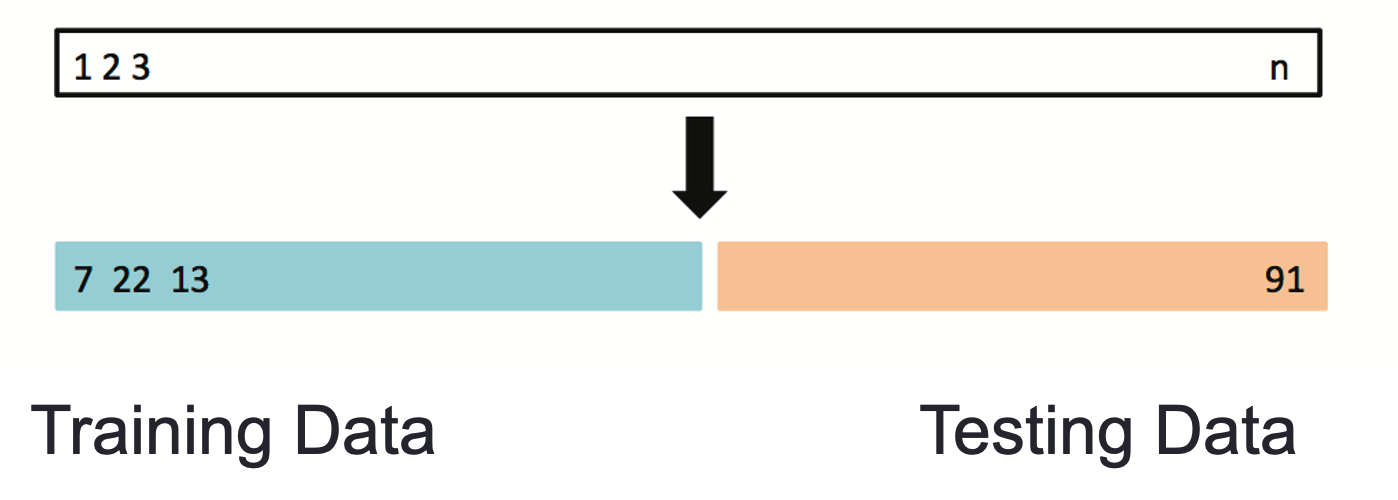
\includegraphics[scale=0.4]{figures/fig51.png}
       \end{figure}

\end{frame}

%----------------------------------------------------------------------%
\begin{frame}[fragile]
\frametitle{The Validation Set Approach}
\begin{itemize}
\item Model $y=f(x) +u$ where $f$ is a polynomial of degree $p^*$. 
\scriptsize
\item Left: Validation error rate for a single split 
\item Right: Validation method repeated 10 times, each time the split is done randomly! 
\item  There is a lot of variability among the MSE’s… Not good! We need more stable methods!
\end{itemize}


 \begin{figure}[H] \centering
            \captionsetup{justification=centering}
              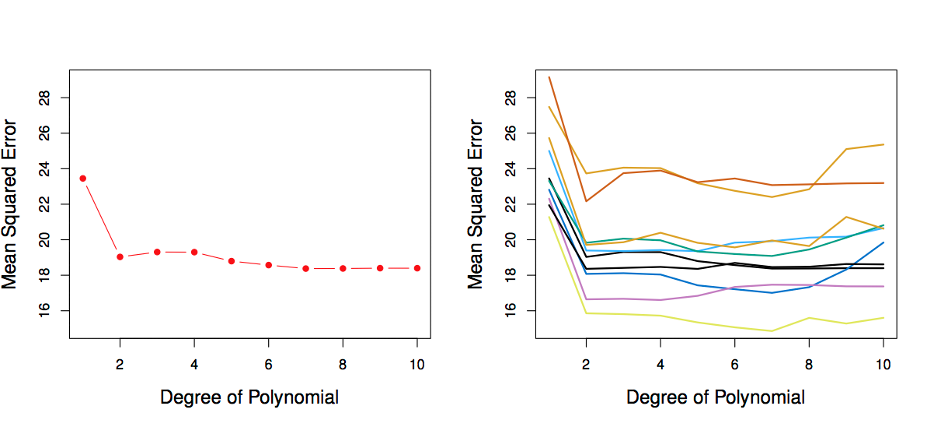
\includegraphics[scale=0.7]{figures/fig52.png}
       \end{figure}
\end{frame}
%----------------------------------------------------------------------%
\begin{frame}[fragile]
\frametitle{The Validation Set Approach}

\begin{itemize}
  \item Advantages:
  \medskip
    \begin{itemize}
      \item Simple
      \medskip
      \item Easy to implement
      \medskip
    \end{itemize}
  \item Disadvantages:
  \medskip
    \begin{itemize}
      \item The validation MSE can be highly variable
      \medskip
      \item  Only a subset of observations are used to fit the model (training data). Statistical methods tend to perform worse when trained on fewer observations
\end{itemize}
\end{itemize}

\end{frame}
%----------------------------------------------------------------------%
\subsection{LOOCV}
%----------------------------------------------------------------------%
\begin{frame}[fragile]
\frametitle{Leave-One-Out Cross Validation (LOOCV)}

\begin{itemize}
\item This method is similar to the Validation Set Approach, but it tries to address the latter’s disadvantages 
\end{itemize}

 \begin{figure}[H] \centering
            \captionsetup{justification=centering}
              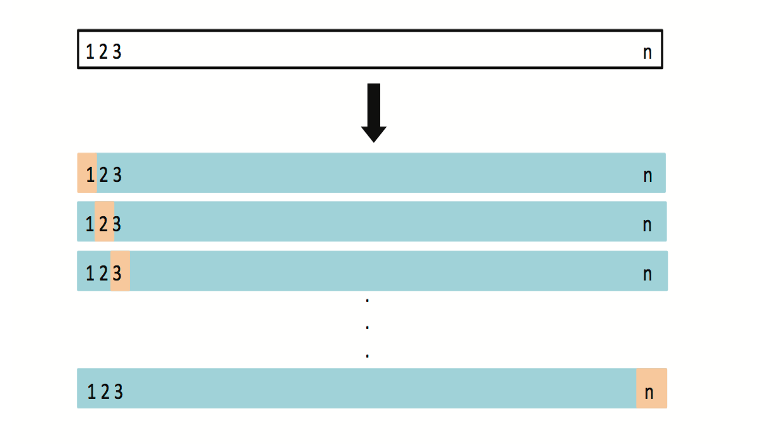
\includegraphics[scale=0.7]{figures/fig53.png}
       \end{figure}


\end{frame}
%----------------------------------------------------------------------%
\subsection{K-fold Cross-Validation}
%----------------------------------------------------------------------%
\begin{frame}[fragile]
\frametitle{K-fold Cross-Validation}
\begin{itemize}
\item LOOCV is computationally intensive, so we can run k-fold Cross Validation instead
\end{itemize}


 \begin{figure}[H] \centering
            \captionsetup{justification=centering}
              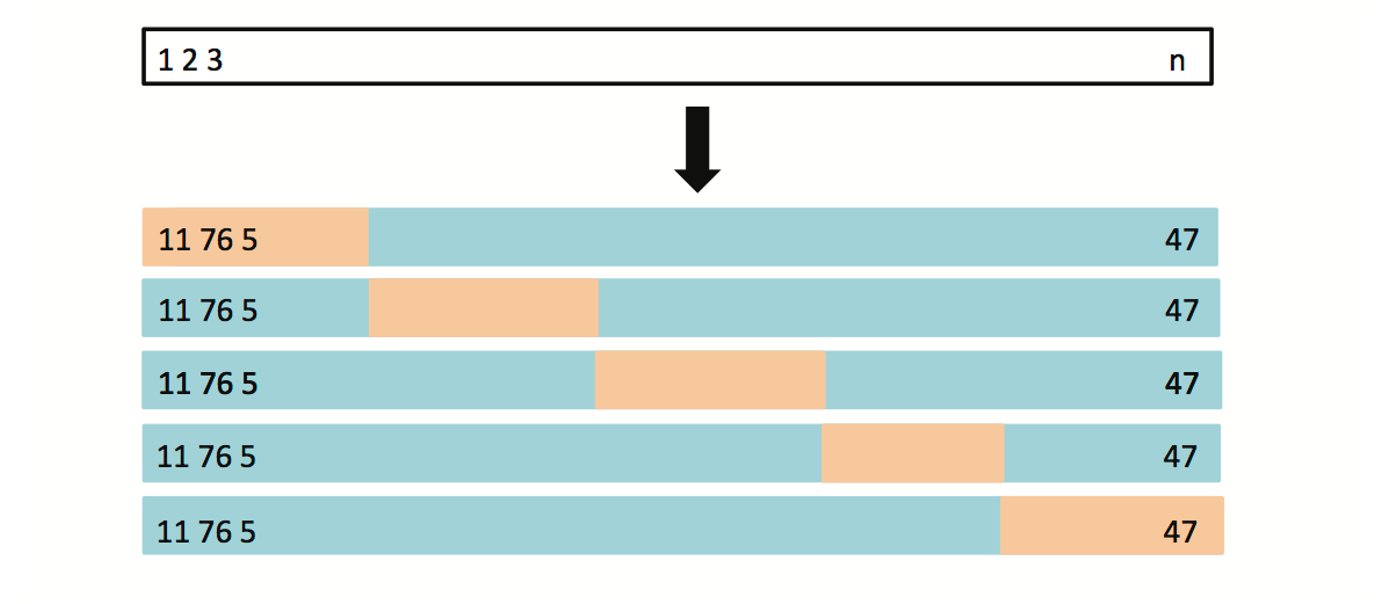
\includegraphics[scale=0.5]{figures/fig55.png}
       \end{figure}



\end{frame}
%----------------------------------------------------------------------%
\begin{frame}[fragile]
\frametitle{K-fold Cross-Validation}

\begin{itemize}
  \item Split the data into K parts $(N=\sum_{j=1}^K n_j)$
  \medskip
  \item Fit the model leaving out one of the folds $\rightarrow$ $f_{-k}(x)$
  \medskip
  \item Calculate the prediction error in the left out fold 
  \begin{align}
  \bar{err_j}=MSE_j=\frac{1}{n_j}\sum L(y_j^k,\hat y_{-j})
  \end{align}
  \medskip
\item Average these out

\begin{align}
CV_{(k)}=\frac{1}{k}\sum_{j=1}^k \bar{err_j}= \frac{1}{k}\sum_{j=1}^k MSE_j
\end{align}
\end{itemize}

\end{frame}
%----------------------------------------------------------------------%
\begin{frame}[fragile]
\frametitle{K-fold Cross-Validation}
\begin{itemize}
  \scriptsize
\item Left: LOOCV  error curve
\item Right: 10-fold CV was run many times, and the figure shows the slightly different CV error rates
\item LOOCV is a special case of k-fold, where k = n
\item They are both stable, but LOOCV (generally) is more computationally intensive! 
\end{itemize}

        \begin{figure}[H] \centering
            \captionsetup{justification=centering}
              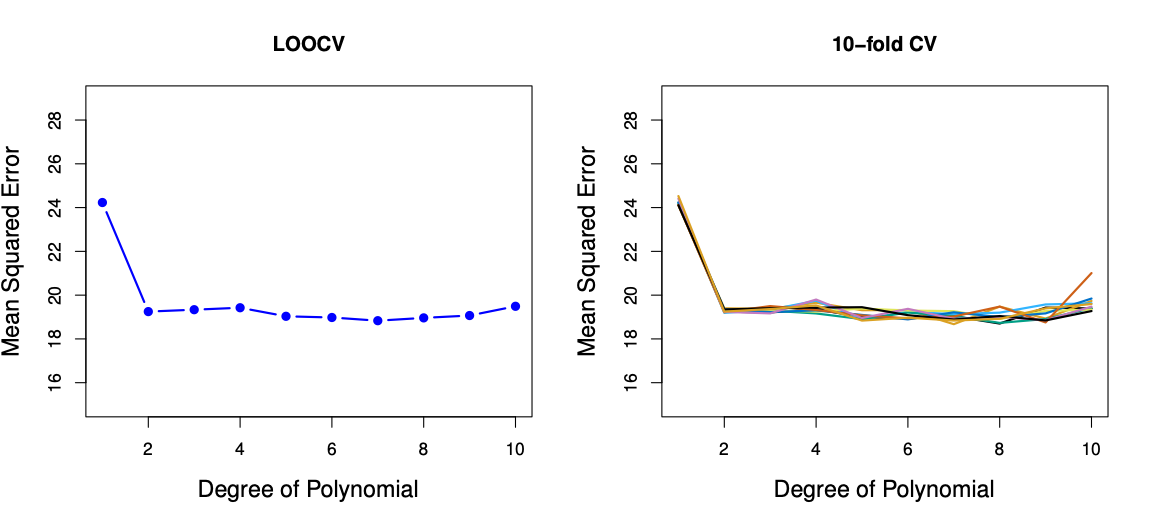
\includegraphics[scale=0.5]{figures/fig54.png}
       \end{figure}
\end{frame}


%----------------------------------------------------------------------%
\begin{frame}[fragile]
\frametitle{K-fold Cross-Validation for Model Selection}

\begin{itemize}
  \item Let's suppose that $\alpha$ parametrizes the complexity of a model
  \medskip
  \item In our examples $\alpha$ would be the degree of the polynomial 
  \medskip
  \item First we compute the CV over an grid of $\alpha$, and then choose the minimum

\end{itemize}
\begin{align}
\underset{\alpha}{min} \, CV_{(k)}(\alpha)
\end{align}

        \begin{figure}[H] \centering
            \captionsetup{justification=centering}
              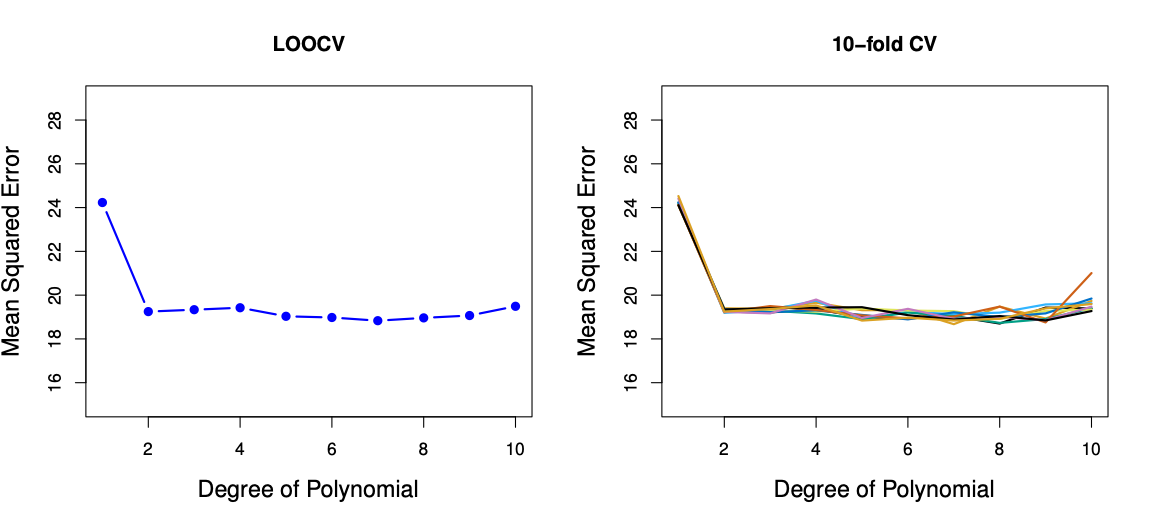
\includegraphics[scale=0.5]{figures/fig54.png}
       \end{figure}

\end{frame}

%----------------------------------------------------------------------%
\begin{frame}[fragile]
\frametitle{Bias- Variance Trade-off for k-fold CV}

\begin{itemize}
  \item Bias:
  \medskip
    \begin{itemize}
      \item Validation set approach tends to overestimate the test error set (less data, worst fit)
      \item LOOCV, adds more data $\rightarrow$ less bias of the test error
      \item K-fold an intermediate state
    \end{itemize}
    \item Variance:
    \begin{itemize}
      \item LOOCV we average the outputs of n fitted models, each is trained in almost identical set of observations $\rightarrow$ highly (positively) correlated
      \item K-fold this correlation is smaller, we are averaging the output of k fitted model that are somewhat less correlated
    \end{itemize}
    \medskip
  \item Thus, there is a trade-off between what to use
  \medskip
    \begin{itemize}
      \item We tend to use k-fold CV with (K = 5 and K = 10)
      \item It has been empirically shown that they yield test error rate estimates that suffer neither from excessively high bias, nor from very high variance Kohavi (1995)
    \end{itemize}
\end{itemize}


\end{frame}



%----------------------------------------------------------------------%
\begin{frame}[fragile]
\frametitle{Spatial K-fold Cross-Validation }

\begin{itemize}
  \scriptsize
  \item 'First law' of geography states that points close to each other are, generally, more similar than points further away
  \item Points are not statistically independent because training and test points in conventional CV are often too close to each other 
  \item To alleviate this problem `spatial partitioning' is used to split the observations into spatially disjointed subsets 
\end{itemize}

 \begin{figure}[H] \centering
            \captionsetup{justification=centering}
              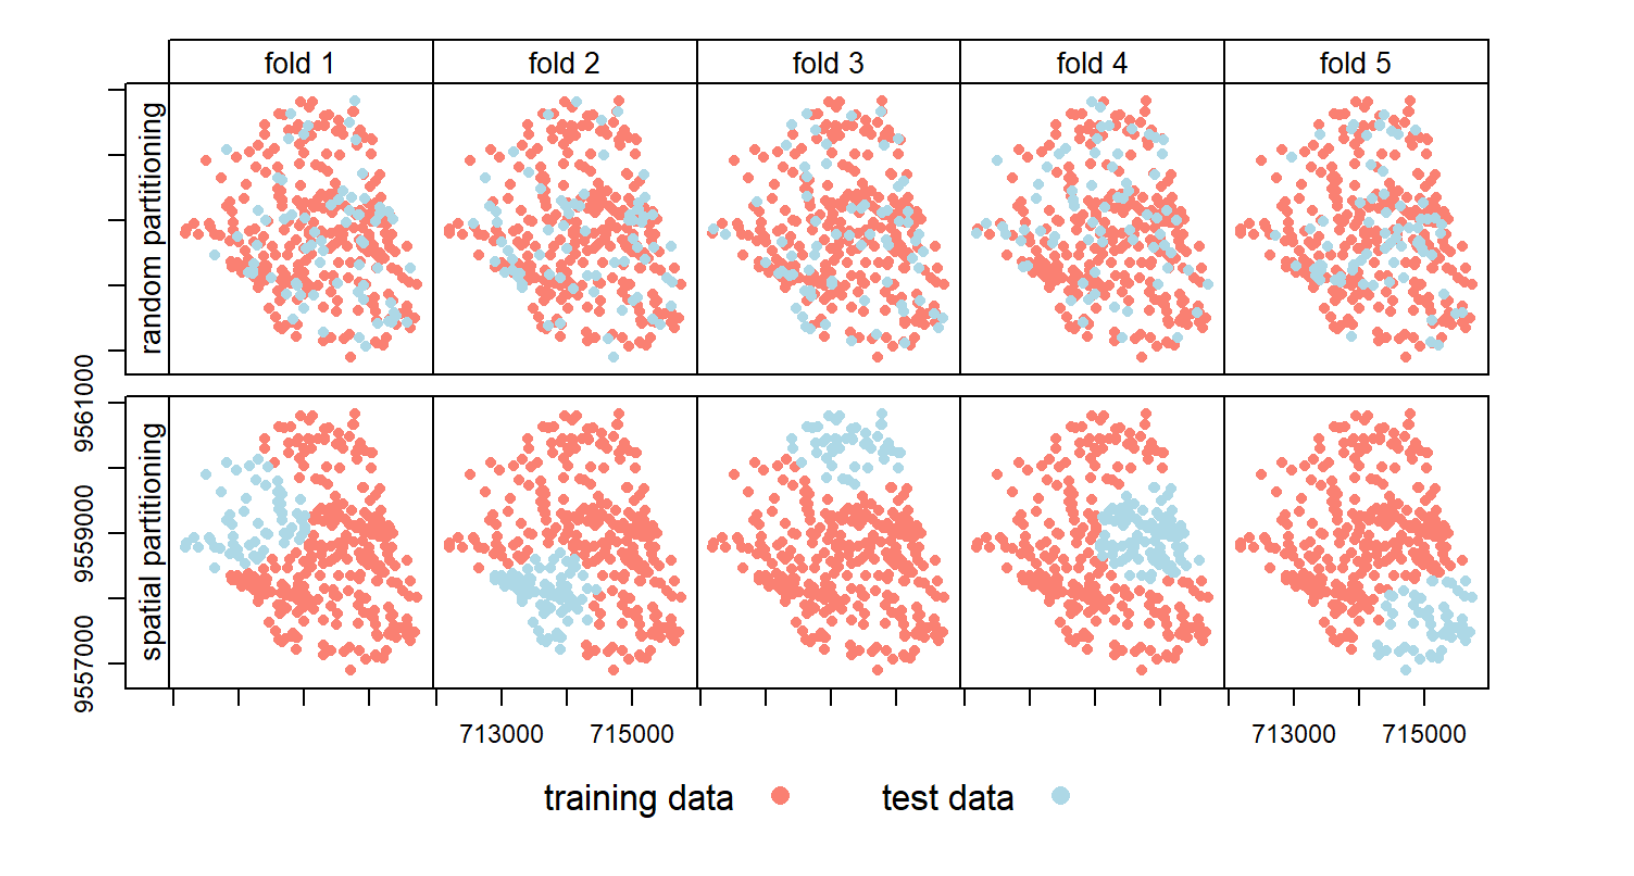
\includegraphics[scale=0.3]{figures/fig113.png}
       \end{figure}

\end{frame}

%----------------------------------------------------------------------%
\begin{frame}
\frametitle{Review \& Next Steps}
  
\begin{itemize} 
    \item Today:
    \medskip
    \begin{itemize} 
         \item Overfit and out of Sample Prediction
         \medskip
         \item Resampling Methods 
        \begin{itemize}  
            \item Validation Set Approach 
            \medskip
            \item LOOCV
            \medskip
            \item K-fold Cross-Validation
      \end{itemize}
    \end{itemize}
  	\bigskip  

	\item  Next class: Model selection and Regularization


\bigskip  
\item Questions? Questions about software? 

\end{itemize}
\end{frame}

%----------------------------------------------------------------------%
\section{Further Readings}
%----------------------------------------------------------------------%
\begin{frame}
\frametitle{Further Readings}

\begin{itemize}


  \item Friedman, J., Hastie, T., \& Tibshirani, R. (2001). The elements of statistical learning (Vol. 1, No. 10). New York: Springer series in statistics.
  \medskip
  \item James, G., Witten, D., Hastie, T., \& Tibshirani, R. (2013). An introduction to statistical learning (Vol. 112, p. 18). New York: springer.
  \medskip
    \item Kohavi, R. (1995). A study of cross-validation and bootstrap for accuracy estimation and model selection. In Ijcai (Vol. 14, No. 2, pp. 1137-1145).
  \medskip
  \item Lovelace, R., Nowosad, J., \& Muenchow, J. (2019). Geocomputation with R. CRC Press. (Chapters 2 \& 6)
\end{itemize}

\end{frame}






%----------------------------------------------------------------------%
%----------------------------------------------------------------------%
\end{document}
%----------------------------------------------------------------------%
%----------------------------------------------------------------------%

